% -*- Mode:TeX -*-

%% IMPORTANT: The official thesis specifications are available at:
%%            http://libraries.mit.edu/archives/thesis-specs/
%%
%%            Please verify your thesis' formatting and copyright
%%            assignment before submission.  If you notice any
%%            discrepancies between these templates and the 
%%            MIT Libraries' specs, please let us know
%%            by e-mailing thesis@mit.edu

%% The documentclass options along with the pagestyle can be used to generate
%% a technical report, a draft copy, or a regular thesis.  You may need to
%% re-specify the pagestyle after you \include  cover.tex.  For more
%% information, see the first few lines of mitthesis.cls. 

%\documentclass[12pt,vi,twoside]{mitthesis}
%%
%%  If you want your thesis copyright to you instead of MIT, use the
%%  ``vi'' option, as above.
%%
\documentclass[12pt,twoside,leftblank]{mitthesis}
%%
%% If you want blank pages before new chapters to be labelled ``This
%% Page Intentionally Left Blank'', use the ``leftblank'' option, as
%% above. 

%\documentclass[12pt,twoside]{mitthesis}
\usepackage{lgrind}
\usepackage{url}
%% These have been added at the request of the MIT Libraries, because
%% some PDF conversions mess up the ligatures.  -LB, 1/22/2014
\usepackage{cmap}
\usepackage[T1]{fontenc}
\pagestyle{plain}

%% This bit allows you to either specify only the files which you wish to
%% process, or `all' to process all files which you \include.
%% Krishna Sethuraman (1990).

%\typein [\files]{Enter file names to process, (chap1,chap2 ...), or `all' to
%process all files:}
%\def\all{all}
%\ifx\files\all \typeout{Including all files.} \else \typeout{Including only \files.} \includeonly{\files} \fi

\begin{document}

% -*-latex-*-
% 
% For questions, comments, concerns or complaints:
% thesis@mit.edu
% 
%
% $Log: cover.tex,v $
% Revision 1.8  2008/05/13 15:02:15  jdreed
% Degree month is June, not May.  Added note about prevdegrees.
% Arthur Smith's title updated
%
% Revision 1.7  2001/02/08 18:53:16  boojum
% changed some \newpages to \cleardoublepages
%
% Revision 1.6  1999/10/21 14:49:31  boojum
% changed comment referring to documentstyle
%
% Revision 1.5  1999/10/21 14:39:04  boojum
% *** empty log message ***
%
% Revision 1.4  1997/04/18  17:54:10  othomas
% added page numbers on abstract and cover, and made 1 abstract
% page the default rather than 2.  (anne hunter tells me this
% is the new institute standard.)
%
% Revision 1.4  1997/04/18  17:54:10  othomas
% added page numbers on abstract and cover, and made 1 abstract
% page the default rather than 2.  (anne hunter tells me this
% is the new institute standard.)
%
% Revision 1.3  93/05/17  17:06:29  starflt
% Added acknowledgements section (suggested by tompalka)
% 
% Revision 1.2  92/04/22  13:13:13  epeisach
% Fixes for 1991 course 6 requirements
% Phrase "and to grant others the right to do so" has been added to 
% permission clause
% Second copy of abstract is not counted as separate pages so numbering works
% out
% 
% Revision 1.1  92/04/22  13:08:20  epeisach

% NOTE:
% These templates make an effort to conform to the MIT Thesis specifications,
% however the specifications can change.  We recommend that you verify the
% layout of your title page with your thesis advisor and/or the MIT 
% Libraries before printing your final copy.
\title{Centralized Storage and Analysis of Machine Learning Operations}

\author{Harihar G. Subramanyam}
% If you wish to list your previous degrees on the cover page, use the 
% previous degrees command:
%       \prevdegrees{A.A., Harvard University (1985)}
% You can use the \\ command to list multiple previous degrees
%       \prevdegrees{B.S., University of California (1978) \\
%                    S.M., Massachusetts Institute of Technology (1981)}
\department{Department of Electrical Engineering and Computer Science}

% If the thesis is for two degrees simultaneously, list them both
% separated by \and like this:
% \degree{Doctor of Philosophy \and Master of Science}
\degree{Master of Engineering in Electrical Engineering and Computer Science}

% As of the 2007-08 academic year, valid degree months are September, 
% February, or June.  The default is June.
\degreemonth{February}
\degreeyear{2017}
\thesisdate{December 16, 2016}

%% By default, the thesis will be copyrighted to MIT.  If you need to copyright
%% the thesis to yourself, just specify the `vi' documentclass option.  If for
%% some reason you want to exactly specify the copyright notice text, you can
%% use the \copyrightnoticetext command.  
%\copyrightnoticetext{\copyright IBM, 1990.  Do not open till Xmas.}

% If there is more than one supervisor, use the \supervisor command
% once for each.
\supervisor{Samuel Madden}{Professor, EECS}

% This is the department committee chairman, not the thesis committee
% chairman.  You should replace this with your Department's Committee
% Chairman.
\chairman{Christopher Terman}{Chairman, Department Committee on Graduate Theses}

% Make the titlepage based on the above information.  If you need
% something special and can't use the standard form, you can specify
% the exact text of the titlepage yourself.  Put it in a titlepage
% environment and leave blank lines where you want vertical space.
% The spaces will be adjusted to fill the entire page.  The dotted
% lines for the signatures are made with the \signature command.
\maketitle

% The abstractpage environment sets up everything on the page except
% the text itself.  The title and other header material are put at the
% top of the page, and the supervisors are listed at the bottom.  A
% new page is begun both before and after.  Of course, an abstract may
% be more than one page itself.  If you need more control over the
% format of the page, you can use the abstract environment, which puts
% the word "Abstract" at the beginning and single spaces its text.

%% You can either \input (*not* \include) your abstract file, or you can put
%% the text of the abstract directly between the \begin{abstractpage} and
%% \end{abstractpage} commands.

% First copy: start a new page, and save the page number.
\cleardoublepage
% Uncomment the next line if you do NOT want a page number on your
% abstract and acknowledgments pages.
% \pagestyle{empty}
\setcounter{savepage}{\thepage}
\begin{abstractpage}
% $Log: abstract.tex,v $
% Revision 1.1  93/05/14  14:56:25  starflt
% Initial revision
% 
% Revision 1.1  90/05/04  10:41:01  lwvanels
% Initial revision
% 
%
%% The text of your abstract and nothing else (other than comments) goes here.
%% It will be single-spaced and the rest of the text that is supposed to go on
%% the abstract page will be generated by the abstractpage environment.  This
%% file should be \input (not \include 'd) from cover.tex.
In this thesis, I designed and implemented a compiler which performs
optimizations that reduce the number of low-level floating point operations
necessary for a specific task; this involves the optimization of chains of
floating point operations as well as the implementation of a ``fixed'' point
data type that allows some floating point operations to simulated with integer
arithmetic.  The source language of the compiler is a subset of C, and the
destination language is assembly language for a micro-floating point CPU.  An
instruction-level simulator of the CPU was written to allow testing of the
code.  A series of test pieces of codes was compiled, both with and without
optimization, to determine how effective these optimizations were.

\end{abstractpage}

% Additional copy: start a new page, and reset the page number.  This way,
% the second copy of the abstract is not counted as separate pages.
% Uncomment the next 6 lines if you need two copies of the abstract
% page.
% \setcounter{page}{\thesavepage}
% \begin{abstractpage}
% % $Log: abstract.tex,v $
% Revision 1.1  93/05/14  14:56:25  starflt
% Initial revision
% 
% Revision 1.1  90/05/04  10:41:01  lwvanels
% Initial revision
% 
%
%% The text of your abstract and nothing else (other than comments) goes here.
%% It will be single-spaced and the rest of the text that is supposed to go on
%% the abstract page will be generated by the abstractpage environment.  This
%% file should be \input (not \include 'd) from cover.tex.
In this thesis, I designed and implemented a compiler which performs
optimizations that reduce the number of low-level floating point operations
necessary for a specific task; this involves the optimization of chains of
floating point operations as well as the implementation of a ``fixed'' point
data type that allows some floating point operations to simulated with integer
arithmetic.  The source language of the compiler is a subset of C, and the
destination language is assembly language for a micro-floating point CPU.  An
instruction-level simulator of the CPU was written to allow testing of the
code.  A series of test pieces of codes was compiled, both with and without
optimization, to determine how effective these optimizations were.

% \end{abstractpage}

\cleardoublepage

\section*{Acknowledgments}

This is the acknowledgements section.  You should replace this with your
own acknowledgements.

%%%%%%%%%%%%%%%%%%%%%%%%%%%%%%%%%%%%%%%%%%%%%%%%%%%%%%%%%%%%%%%%%%%%%%
% -*-latex-*-

% Some departments (e.g. 5) require an additional signature page.  See
% signature.tex for more information and uncomment the following line if
% applicable.
% % -*- Mode:TeX -*-
%
% Some departments (e.g. Chemistry) require an additional cover page
% with signatures of the thesis committee.  Please check with your
% thesis advisor or other appropriate person to determine if such a 
% page is required for your thesis.  
%
% If you choose not to use the "titlepage" environment, a \newpage
% commands, and several \vspace{\fill} commands may be necessary to
% achieve the required spacing.  The \signature command is defined in
% the "mitthesis" class
%
% The following sample appears courtesy of Ben Kaduk <kaduk@mit.edu> and
% was used in his June 2012 doctoral thesis in Chemistry. 

\begin{titlepage}
\begin{large}
This doctoral thesis has been examined by a Committee of the Department
of Chemistry as follows:

\signature{Professor Jianshu Cao}{Chairman, Thesis Committee \\
   Professor of Chemistry}

\signature{Professor Troy Van Voorhis}{Thesis Supervisor \\
   Associate Professor of Chemistry}

\signature{Professor Robert W. Field}{Member, Thesis Committee \\
   Haslam and Dewey Professor of Chemistry}
\end{large}
\end{titlepage}


\pagestyle{plain}
  % -*- Mode:TeX -*-
%% This file simply contains the commands that actually generate the table of
%% contents and lists of figures and tables.  You can omit any or all of
%% these files by simply taking out the appropriate command.  For more
%% information on these files, see appendix C.3.3 of the LaTeX manual. 
\tableofcontents
\newpage
\listoffigures
\newpage
\listoftables


%% This is an example first chapter.  You should put chapter/appendix that you
%% write into a separate file, and add a line \include{yourfilename} to
%% main.tex, where `yourfilename.tex' is the name of the chapter/appendix file.
%% You can process specific files by typing their names in at the 
%% \files=
%% prompt when you run the file main.tex through LaTeX.
\chapter{Introduction}

Micro-optimization is a technique to reduce the overall operation count of
floating point operations.  In a standard floating point unit, floating
point operations are fairly high level, such as ``multiply'' and ``add'';
in a micro floating point unit ($\mu$FPU), these have been broken down into
their constituent low-level floating point operations on the mantissas and
exponents of the floating point numbers.

Chapter two describes the architecture of the $\mu$FPU unit, and the
motivations for the design decisions made.

Chapter three describes the design of the compiler, as well as how the
optimizations discussed in section~\ref{ch1:opts} were implemented.

Chapter four describes the purpose of test code that was compiled, and which
statistics were gathered by running it through the simulator.  The purpose
is to measure what effect the micro-optimizations had, compared to
unoptimized code.  Possible future expansions to the project are also
discussed.

\section{Motivations for micro-optimization}

The idea of micro-optimization is motivated by the recent trends in computer
architecture towards low-level parallelism and small, pipelineable
instruction sets \cite{patterson:risc,rad83}.  By getting rid of more
complex instructions and concentrating on optimizing frequently used
instructions, substantial increases in performance were realized.

Another important motivation was the trend towards placing more of the
burden of performance on the compiler.  Many of the new architectures depend
on an intelligent, optimizing compiler in order to realize anywhere near
their peak performance
\cite{ellis:bulldog,pet87,coutant:precision-compilers}.  In these cases, the
compiler not only is responsible for faithfully generating native code to
match the source language, but also must be aware of instruction latencies,
delayed branches, pipeline stages, and a multitude of other factors in order
to generate fast code \cite{gib86}.

Taking these ideas one step further, it seems that the floating point
operations that are normally single, large instructions can be further broken
down into smaller, simpler, faster instructions, with more control in the
compiler and less in the hardware.  This is the idea behind a
micro-optimizing FPU; break the floating point instructions down into their
basic components and use a small, fast implementation, with a large part of
the burden of hardware allocation and optimization shifted towards
compile-time.

Along with the hardware speedups possible by using a $\mu$FPU, there are
also optimizations that the compiler can perform on the code that is
generated.  In a normal sequence of floating point operations, there are
many hidden redundancies that can be eliminated by allowing the compiler to
control the floating point operations down to their lowest level.  These
optimizations are described in detail in section~\ref{ch1:opts}.

\section{Description of micro-optimization}\label{ch1:opts}

In order to perform a sequence of floating point operations, a normal FPU
performs many redundant internal shifts and normalizations in the process of
performing a sequence of operations.  However, if a compiler can
decompose the floating point operations it needs down to the lowest level,
it then can optimize away many of these redundant operations.  

If there is some additional hardware support specifically for
micro-optimization, there are additional optimizations that can be
performed.  This hardware support entails extra ``guard bits'' on the
standard floating point formats, to allow several unnormalized operations to
be performed in a row without the loss information\footnote{A description of
the floating point format used is shown in figures~\ref{exponent-format}
and~\ref{mantissa-format}.}.  A discussion of the mathematics behind
unnormalized arithmetic is in appendix~\ref{unnorm-math}.

The optimizations that the compiler can perform fall into several categories:

\subsection{Post Multiply Normalization}

When more than two multiplications are performed in a row, the intermediate
normalization of the results between multiplications can be eliminated.
This is because with each multiplication, the mantissa can become
denormalized by at most one bit.  If there are guard bits on the mantissas
to prevent bits from ``falling off'' the end during multiplications, the
normalization can be postponed until after a sequence of several
multiplies\footnote{Using unnormalized numbers for math is not a new idea; a
good example of it is the Control Data CDC 6600, designed by Seymour Cray.
\cite{thornton:cdc6600} The CDC 6600 had all of its instructions performing
unnormalized arithmetic, with a separate {\tt NORMALIZE} instruction.}.

% This is an example of how you would use tgrind to include an example
% of source code; it is commented out in this template since the code
% example file does not exist.  To use it, you need to remove the '%' on the
% beginning of the line, and insert your own information in the call.
%
%\tagrind[htbp]{code/pmn.s.tex}{Post Multiply Normalization}{opt:pmn}

As you can see, the intermediate results can be multiplied together, with no
need for intermediate normalizations due to the guard bit.  It is only at
the end of the operation that the normalization must be performed, in order
to get it into a format suitable for storing in memory\footnote{Note that
for purposed of clarity, the pipeline delays were considered to be 0, and
the branches were not delayed.}.

\subsection{Block Exponent}

In a unoptimized sequence of additions, the sequence of operations is as
follows for each pair of numbers ($m_1$,$e_1$) and ($m_2$,$e_2$).
\begin{enumerate}
  \item Compare $e_1$ and $e_2$.
  \item Shift the mantissa associated with the smaller exponent $|e_1-e_2|$
        places to the right.
  \item Add $m_1$ and $m_2$.
  \item Find the first one in the resulting mantissa.
  \item Shift the resulting mantissa so that normalized
  \item Adjust the exponent accordingly.
\end{enumerate}

Out of 6 steps, only one is the actual addition, and the rest are involved
in aligning the mantissas prior to the add, and then normalizing the result
afterward.  In the block exponent optimization, the largest mantissa is
found to start with, and all the mantissa's shifted before any additions
take place.  Once the mantissas have been shifted, the additions can take
place one after another\footnote{This requires that for n consecutive
additions, there are $\log_{2}n$ high guard bits to prevent overflow.  In
the $\mu$FPU, there are 3 guard bits, making up to 8 consecutive additions
possible.}.  An example of the Block Exponent optimization on the expression
X = A + B + C is given in figure~\ref{opt:be}.

% This is an example of how you would use tgrind to include an example
% of source code; it is commented out in this template since the code
% example file does not exist.  To use it, you need to remove the '%' on the
% beginning of the line, and insert your own information in the call.
%
%\tgrind[htbp]{code/be.s.tex}{Block Exponent}{opt:be}

\section{Integer optimizations}

As well as the floating point optimizations described above, there are
also integer optimizations that can be used in the $\mu$FPU.  In concert
with the floating point optimizations, these can provide a significant
speedup.  

\subsection{Conversion to fixed point}

Integer operations are much faster than floating point operations; if it is
possible to replace floating point operations with fixed point operations,
this would provide a significant increase in speed.

This conversion can either take place automatically or or based on a
specific request from the programmer.  To do this automatically, the
compiler must either be very smart, or play fast and loose with the accuracy
and precision of the programmer's variables.  To be ``smart'', the computer
must track the ranges of all the floating point variables through the
program, and then see if there are any potential candidates for conversion
to floating point.  This technique is discussed further in
section~\ref{range-tracking}, where it was implemented.

The other way to do this is to rely on specific hints from the programmer
that a certain value will only assume a specific range, and that only a
specific precision is desired.  This is somewhat more taxing on the
programmer, in that he has to know the ranges that his values will take at
declaration time (something normally abstracted away), but it does provide
the opportunity for fine-tuning already working code.

Potential applications of this would be simulation programs, where the
variable represents some physical quantity; the constraints of the physical
system may provide bounds on the range the variable can take.
\subsection{Small Constant Multiplications}

One other class of optimizations that can be done is to replace
multiplications by small integer constants into some combination of
additions and shifts.  Addition and shifting can be significantly faster
than multiplication.  This is done by using some combination of
\begin{eqnarray*}
a_i & = & a_j + a_k \\
a_i & = & 2a_j + a_k \\
a_i & = & 4a_j + a_k \\
a_i & = & 8a_j + a_k \\
a_i & = & a_j - a_k \\
a_i & = & a_j \ll m \mbox{shift}
\end{eqnarray*}
instead of the multiplication.  For example, to multiply $s$ by 10 and store
the result in $r$, you could use:
\begin{eqnarray*}
r & = & 4s + s\\
r & = & r + r
\end{eqnarray*}
Or by 59:
\begin{eqnarray*}
t & = & 2s + s \\
r & = & 2t + s \\
r & = & 8r + t
\end{eqnarray*}
Similar combinations can be found for almost all of the smaller
integers\footnote{This optimization is only an ``optimization'', of course,
when the amount of time spent on the shifts and adds is less than the time
that would be spent doing the multiplication.  Since the time costs of these
operations are known to the compiler in order for it to do scheduling, it is
easy for the compiler to determine when this optimization is worth using.}.
\cite{magenheimer:precision}

\section{Other optimizations}

\subsection{Low-level parallelism}

The current trend is towards duplicating hardware at the lowest level to
provide parallelism\footnote{This can been seen in the i860; floating point
additions and multiplications can proceed at the same time, and the RISC
core be moving data in and out of the floating point registers and providing
flow control at the same time the floating point units are active. \cite{byte:i860}}

Conceptually, it is easy to take advantage to low-level parallelism in the
instruction stream by simply adding more functional units to the $\mu$FPU,
widening the instruction word to control them, and then scheduling as many
operations to take place at one time as possible.

However, simply adding more functional units can only be done so many times;
there is only a limited amount of parallelism directly available in the
instruction stream, and without it, much of the extra resources will go to
waste.  One process used to make more instructions potentially schedulable
at any given time is ``trace scheduling''.  This technique originated in the
Bulldog compiler for the original VLIW machine, the ELI-512.
\cite{ellis:bulldog,colwell:vliw}  In trace scheduling, code can be
scheduled through many basic blocks at one time, following a single
potential ``trace'' of program execution.  In this way, instructions that
{\em might\/} be executed depending on a conditional branch further down in
the instruction stream are scheduled, allowing an increase in the potential
parallelism.  To account for the cases where the expected branch wasn't
taken, correction code is inserted after the branches to undo the effects of
any prematurely executed instructions.

\subsection{Pipeline optimizations}

In addition to having operations going on in parallel across functional
units, it is also typical to have several operations in various stages of
completion in each unit.  This pipelining allows the throughput of the
functional units to be increased, with no increase in latency.

There are several ways pipelined operations can be optimized.  On the
hardware side, support can be added to allow data to be recirculated back
into the beginning of the pipeline from the end, saving a trip through the
registers.  On the software side, the compiler can utilize several tricks to
try to fill up as many of the pipeline delay slots as possible, as
seendescribed by Gibbons. \cite{gib86}



%\chapter{Related Work}

\section{Machine Learning}
There are many classes of problems that machine learning can be used to solve, such
as the following~\cite{introtoml}:

\begin{itemize}
  \item \textbf{Supervised Learning}: Predict a real valued output (regression)
    or select one of $C$ predefined categorical outputs (classification)
    for a given input vector. This also includes problems like anomaly detection,
    ranking, and regression.
  \item \textbf{Unsupervised Learning}: Find structure or regularity in a given
    set of input vectors. This includes problems like density estimation and 
    clustering.
  \item \textbf{Reinforcement Learning}: Develop a policy that allows an agent
    to observe the state of its environment and take the actions that will 
    achieve a large cumulative reward in the long run~\cite{introtorl}.
\end{itemize}

ModelDB S+C can store operations and models for supervised
and unsupervised learning problems. Reinforcement learning, however, is out
of scope for this thesis.

For a supervised learning problem, suppose there is a dataset $\mathcal{D}$ that
consists of $n$ pairs of $(\textbf{x}^{(i)}, y^{(i)})$. There is a
pair for each $i \in \{{1...n}\}$. $\textbf{x}^{(i)}$ is a $p$-dimensional feature
vector that decribes the $i^{th}$ example. So, $\textbf{x}^{(i)} \in \mathbb{R}^{p}$. 
$y^{(i)}$ is either the class label associated with the $i^{th}$ example or
the regression target for that example. That is, $y^{(i)} \in \{1...C\}$ for classification
and $y^{(i)} \in \mathbb{R}$ for regression. The $\textbf{x}^{(i)}$ vectors
can also be expressed as a $n \times p$ matrix $\textbf{X}$.

A machine learning model is a function $f(\textbf{x}; \boldsymbol{\theta})$ where
$\boldsymbol{\theta}$ is a vector of model parameters (e.g. the weights of a linear regression
model or the encoded splits of a decision tree model). This function accepts an 
input vector $\textbf{x} \in \mathbb{R}^{p}$ and produces a real output (for regression)
or probability of being in a specific class (for classification).

When training a model, it is useful to split the dataset $\mathcal{D}$ into
a training set $\mathcal{D}_{train}$ and testing set $\mathcal{D}_{test}$. This ensures
that the model is evaluated on data it has not seen before. An objective function
$J(\boldsymbol{\theta}, \mathcal{D}_{train})$ is defined and $\boldsymbol{\theta}$ 
is chosen to maximize (or minimize, depending on the formulation) the objective function.

Machine learning also requires some hyperparameters (e.g. maximum depth of decision tree, regularization constant) 
to be set in order to guide the training of the model. One way to pick values for the hyperparameters
is to use a validation set. That is, the dataset $\mathcal{D}$ is broken into three pieces, 
$\mathcal{D}_{train}$, $\mathcal{D}_{validation}$, and $\mathcal{D}_{test}$. For each 
hyperparameter configuration, a model is trained on $\mathcal{D}_{train}$. Then, the model
is evaluated on $\mathcal{D}_{validation}$. Then, the chosen hyperparameter configuration
is the one that yielded the model that performed best on the validation set. 
Using a technique called cross validation can make better use of the data. In 
$k$-fold cross validation, $\mathcal{D}_{train}$ is broken into $k$ pieces (or folds) of roughly
equal size. Then, for a given hyperparameter configuration, a total of $k$ models are trained, each 
trained on all but one of the folds. Each model is evaluated on the fold that was left out of its training,
and the resulting evaluation metrics are aggregated (e.g. averaged) to produce the evaluation
metric for the hyperparameter configuration. The hyperparameter configuration with the
largest evaluation metric is chosen as the best hyperparameter configuration. Then, a final
model is trained on the entire $\mathcal{D}_{train}$ and is then evaluated on $\mathcal{D}_{test}$ 
\cite{deeplearningbook}.

While the above concepts are not exhaustive, they provide an overview of machine learning that is sufficient to
understand the model building process and ModelDB S+C.

\section{Linear and Tree Models}
ModelDB S+C has special support for linear regression, logistic regression, 
decision tree, random forest, and gradient boosted tree models. Therefore, it is worth discussing
these models briefly.

A linear regression model is a function $f(\textbf{x}; \boldsymbol{\theta}) = \boldsymbol{\theta}^{T}\textbf{x}$,
where $\boldsymbol{\theta} \in \mathbb{R}^{p}$. Requiring that all feature vectors have an first entry of 
1 allows the model to incorporate an intercept term.

A logistic regression model is not actually used for regression, it is used for 
binary ($C=2$) classification. Under appropriate assumptions, the logistic 
regression model aims to predict the likelihood that a given input feature vector
belongs to class 1. Concretely, the logistic regression function is: 
$f(\textbf{x}; \boldsymbol{\theta}) = \frac{\exp{\boldsymbol{\theta}^{T}\textbf{x}}}{1 + \exp{\boldsymbol{\theta}^{T}\textbf{x}}}$.
Its output lies between 0 and 1.

A decision tree model partitions the input space into non-overlapping regions, where all
points in the same region are assigned the same value. This value could be a class label
in the case of classification or a real value in the case of regression. For a given input vector,
the decision tree considers a different feature at each internal node. The input vector is forwarded
to a child node based on the value of the feature. This child node, if it is an internal node, then considers another
feature and performs the same process. Eventually, the input vector arrives at a leaf node. Each leaf node corresponds to
a region of the input space, and thus has an associated value (i.e. class label or real number), which is taken
to be the prediction for the input vector. An illustration of this is shown in Figure \ref{fig:sample_decision_tree}.

\begin{figure}
  \centering
  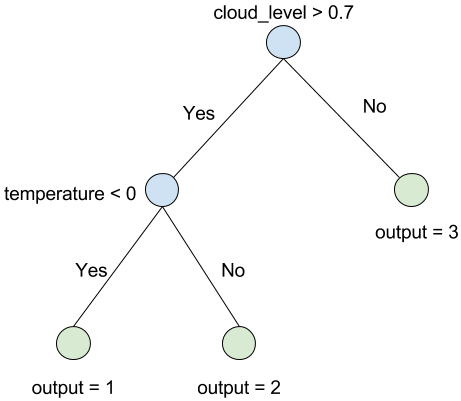
\includegraphics[height=3.0in]{sample_decision_tree}
  \caption{This is a decision tree model that could be used to predict whether the
  weather will be snowy (output 1), rainy (output 2), or neither (output 3) by
  looking at the cloud cover and temperature. The tree first checks if the cloud cover
  is high. If not, then it predicts there will be neither rain nor snow. Otherwise, the
  tree checks if the temperature is below 0. If so, then it predicts snow. Otherwise, it
  predicts rain.}
  \label{fig:sample_decision_tree}
\end{figure}

Random forest models and gradient boosted tree models are both ensembles of decision trees. They just differ in how they
are trained and applied. A random forest model trains many trees in parallel, where each tree is trained on a different bootstrapped
sample of the original dataset and where each split is only allowed to consider a subset of the features. A gradient boosted tree model
trains decision trees iteratively, where each successive decision tree learns to correct the mistakes of the previous trees. Like decision
trees, random forest and gradient boosted tree models can be used for both classification and regression. \cite{introtostatlearn}

These are not the only linear and tree models that are used in practice, but they are models that are supported in Spark.ML. 
Therefore, ModelDB S+C provides additional functionalty for the aforementioned models.

\section{Spark.ML}
Apache Spark \cite{spark} is a cluster computing engine that efficiently performs distributed computation
on data stored in-memory on many different machines. It is built around 
an abstraction called the Resilient Distributed Dataset (RDD). An RDD represents a dataset, its lineage,
and its partitioning. By tracking a dataset's lineage, an RDD allows the dataset to be recreated if it is
lost, thus providing fault tolerance. By tracking the partitioning and lazily performing operations, Spark
uses RDDs to schedule operations intelligently and pipeline them for efficiency.

Spark includes a number of libraries, two of which are relevant for this thesis. The first is Spark SQL,
which builds an abstraction called a DataFrame on top of the RDD abstraction. A DataFrame is simply a table
of data with named, typed columns. The second library
is Spark.ML, which lets users build machine learning models using Spark. Spark.ML lets the user create Transformers
that take an input DataFrame and produce an output DataFrame. It lets users use Estimators, which accept hyperparameters
and a DataFrame and produce a resulting model, which is simply a Transformer. Finally, Spark.ML provides a number
of other classes to support common model building tasks like cross validation and making preprocessing pipelines.

ModelDB S+C is built on three primitives: Transformer, DataFrame, and TransformerSpec, which are all inspired
by Spark SQL and Spark.ML. Transformer and DataFrame match their Spark counterparts, but unlike a Spark Estimator, a 
TransformerSpec simply describes how to create a model, rather than containing the logic for actually training the model.
ModelDB S+C does not train models, so there is no need for it to have model training logic.

The three primitives above, when coupled with ModelDB S+C's Syncable Event abstraction, can express a wide range
of model building operations.

The ModelDB Spark Client is a library designed for Spark.ML. It allows the user to use their existing
Spark.ML code, and with a few minor changes, store all their operations and models in ModelDB Server. 

\section{Machine Learning Libraries}
Since ModelDB Server aims to be library agnostic, it is worth looking at some other popular
machine learning libraries and understanding their abstractions for the model building process.

\subsection{MLI}
MLI \cite{mli} is an API for distributed machine learning. It includes an MLTable abstraction
that is very similar to the DataFrame abstraction in ModelDB S+C. MLI includes two other
tabular abstractions, the LocalMatrix and MLNumericTable, which are more restrictive forms of the
MLTable. MLNumericTable and LocalMatrix make computation easier, but they do not add anything to
the expressive power of MLI.

MLI's Optimizer and Algorithm abstractions help specify the logic for training a model. However,
as stated before, ModelDB S+C does not perform any training of models and thus these abstractions
are not important in the context of ModelDB S+C. That being said, the user can store information
about the algorithms and optimizer used to train a model in the hyperparameters of the model's associated
TransformerSpec.

MLI's Model abstraction maps to the Transformer abstraction in ModelDB S+C. There are two 
key differences between these abstractions. First, a Transformer is more general 
than a Model; it can represent data preprocessors as well as models. Second, a Model
stores the logic for making predictions while a Transformer does not. This is because
ModelDB S+C does not aim to make predictions, just to store and analyze the model building process. However,
the user is able to store serialized models in ModelDB S+C, which can later be deserialized and used to make
predictions.

\subsection{Scikit-learn}
Scikit-learn \cite{scikitlearn} is a machine learning library for Python. It expects data to
be given as matrices (two dimensional arrays in the numpy Python library) and DataFrames (from the Python
Pandas library). Both of these abstractions map nicely to ModelDB S+C's DataFrame.
A matrix can be thought of as a DataFrame where all columns are numeric and where the column names are ignored.

Scikit-learn includes the concept of an Estimator, which contains logic for training a model and stores the hyperparameters.
This maps well to ModelDB S+C's TransformerSpec. The logic for training the model is not necessary for ModelDB S+C. Scikit-learn
also includes Transformer and Predictor concepts. The former is almost identical to ModelDB S+C's Transformer abstraction while the 
latter is simply a more restrictive kind of Transformer.

Finally, Scikit-learn includes abstractions for cross validation and pipelines, much like Spark.ML does. Both of these
model building tasks are represented in ModelDB S+C as Syncable Events.

\subsection{Weka}
Weka \cite{weka} is a machine learning toolkit that includes a user interface targeted for non-expert users.
It represents data as tables, which is very similar to ModelDB S+C's DataFrame.
However, Weka does not include separate abstractions for describing a model and describing the fitting of a model. Instead,
it combines them together in an abstraction called a Scheme. Thus, ModelDB S+C's TransformerSpec and Transformer abstraction
together reflect the same information as a Weka Scheme. Finally, Weka includes pre-processing and post-processing utilities which
map well to ModelDB S+C's Transformer abstraction.

\subsection{Pylearn 2}
Pylearn 2 \cite{pylearn2} is a machine learning library geared towards researchers. It includes the concept of a Dataset, Model,
and TrainingAlgorithm, which are analogous to ModelDB S+C's concepts of a DataFrame, Transformer, and TransformerSpec.
ModelDB S+C's Transformer abstraction is more general than a Model because it can capture both models as well as data preprocessors.
Pylearn 2 also includes abstractions such as Cost and TerminationCriterion. Since ModelDB S+C does not concern itself with the
details of training models, it has no corresponding abstractions and instead allows the data scientist to specify cost and termination criterion
as hyperparameters in a TransformerSpec.

\subsection{Tensorflow}
Tensorflow \cite{tensorflow} is machine learning library that allows users to specify computation graphs, which is
especially useful for training neural network models. It represents data in the form of a Tensor. 
This is actually more general than the DataFrame concept in ModelDB S+C. However, using a tensor abstraction in ModelDB S+C may
add a good deal of complexity to the other abstractions without enabling a great deal of new functionality. 

Tensorflow represents data in the form of a computation graph, where nodes 
called variables use operations along edges to send tensors through the graph.
ModelDB S+C stores a graph, specified by the TransformEvents, where the 
nodes are DataFrames and the edges are Transformers. Tensorflow's computation 
graph is useful for performing efficient training of models. However, since 
ModelDB S+C does not actually do any training of models and instead just 
captures operations like transformations and model-fitting, its graph is 
different than TensorFlow's. Additionally, Tensorflow requires the user to 
specifiy their computation graph up-front in order for
the library to determine how to train the model. ModelDB S+C, on 
the other hand, builds up its graph over time as the user performs operations.

\subsection{Summary}
Thus, ModelDB S+C's abstractions seem to be general enough that there are analogs
in a number of other machine learning libraries. Of the examples above, Tensorflow
is the only one with a significantly different set of abstractions than ModelDB S+C.

\section{Model Building Support Systems}
ModelDB S+C does not actually train any machine learning models and it does not 
make any predictions. Rather, it collects, stores, and analyzes data about 
the model building process. In this way, ModelDB S+C supports the process of
model building rather than performing the process itself. This section describes
other systems that support the model building process.

\subsection{ModelHub}
ModelHub \cite{modelhub} is similar to the overall ModelDB system in that it also
aims to provide a suite of systems like model version control, a command line
toolkit, and a model exploration API, to support the model building process. ModelHub
focuses on deep learning and provides specialized tools for that domain, however, 
while ModelDB is aimed at machine learning models in general. Additionally, while
ModelHub tracks changes made to models, it does not track transformations 
made to datasets like ModelDB S+C does. Finally, ModelHub does not describe
any client libraries or abstractions that allow collecting data about the data
scientist's operations as they are performed. ModelDB Spark Client, on the other hand,
records a wide range of machine learning operations, like random splitting of datasets,
annotating datasets, and creating preprocessing pipelines, as the user does them and
stores them in ModelDB Server.

\subsection{MLDB}
MLDB \cite{mldb} is a system that allows users to create and store machine learning
models as well as datasets in a central database and access them through a REST API. 
While it supports the storage of models, it does not store operations (e.g. random splitting,
pipeline creation) that the user performs. Additionally, there are no client libraries
that can record these operations behind the scenes and send them to the server with
minimal user involvement. Finally, MLDB does not offer an API for querying operations
and gleaning information from them.

\subsection{Azure ML}
Microsoft's Azure Machine Learning \cite{azureml} is a cloud service that allows users
to create machine learning models with a web interface, store them in the cloud, and
access them via web service. Azure Machine Learning requires users to construct a dataflow 
graph indicating their full pre-processing and model training operations before model building
happens. ModelDB S+C, on the other hand, does not ask the user to indicate their full model building
workflow beforehand, and will instead record the operations and models as they appear. ModelDB Server
focuses on storing and analyzing the model building process and allows the user to use another library
(Spark.ML in this thesis) for training models. Azure Machine Learning, on the other hand, requires
that the user use its model training system. Finally ModelDB Spark Client works with a user's existing
Spark.ML code, allowing them to log their operations and models with few code changes. Azure Machine
Learning, on the other hand, requires users to convert significant parts of their code into
dataflow graphs using its proprietary user interface.

\subsection{Velox}
Velox \cite{velox} is a system for low latency serving and management of machine learning models.
While it does support storage of models, it does not store operations performed in model building and it
does not expose APIs for analyzing the model building process.

\subsection{MLBase}
MLBase \cite{mlbase} is a database system with the ability to store and serve machine learning
models. It includes an optimizer that figures out a plan for training a model. Unlike ModelDB S+C,
it does not track and store the operations in the model building process. It also requires users to
specify their model building process using a declarative language with hints for the optimizer. While this
can be useful for non-experts, it reduces the control that a user has over their model building process.
ModelDB S+C on the other hand, only requires a few minor changes to the user's Spark.ML code in order to
store the data associated with the model building process.

\subsection{PMML}
PMML \cite{pmml} is an XML-like markup language for representing machine learning models. While it
can describe a wide range of machine learning models, it cannot represent general model building operations
like ModelDB Server's database does. It is not possible to run queries on PMML either. ModelDB Server, on the other hand,
exposes an API for querying model building operations and stores operation data in a SQL database. PMML can,
however, complement ModelDB Server because a user can choose to store their serialized models in PMML form.

\subsection{Longview}
Longview is a predictive DBMS. It allows users to store machine learning models in a relational database
and access them via a user defined function in their queries. Unlike ModelDB S+C, it
cannot work with a user's existing code, and instead requires them to use Longview for all their
model training. Finally, Longview does not store machine learning operations like ModelDB Server does.

%\chapter{Tables}

\begin{table}
\caption{Armadillos}
\label{arm:table}
\begin{center}
\begin{tabular}{||l|l||}\hline
Armadillos & are \\\hline
our	   & friends \\\hline
\end{tabular}
\end{center}
\end{table}

\clearpage
\newpage

%\chapter{Figures}

\vspace*{-3in}

\begin{figure}
\vspace{2.4in}
\caption{Armadillo slaying lawyer.}
\label{arm:fig1}
\end{figure}
\clearpage
\newpage

\begin{figure}
\vspace{2.4in}
\caption{Armadillo eradicating national debt.}
\label{arm:fig2}
\end{figure}
\clearpage
\newpage

\appendix
%% This defines the bibliography file (main.bib) and the bibliography style.
%% If you want to create a bibliography file by hand, change the contents of
%% this file to a `thebibliography' environment.  For more information 
%% see section 4.3 of the LaTeX manual.
\begin{singlespace}
\bibliography{main}
\bibliographystyle{plain}
\end{singlespace}

\end{document}

